\documentclass[stu,12pt,floatsintext]{apa7}

\usepackage[american]{babel}

\usepackage{csquotes}
\usepackage[style=apa,backend=bibtex]{biblatex}
\DeclareLanguageMapping{american}{american-apa} % Gotta make sure we're patriotic up in here. Seriously, though, there can be local variants to how citations are handled, this sets it to the American idiosyncrasies 
\addbibresource{bibliography.bib} % This is the companion file to the main one you're writing. It contains all of the bibliographic info for your references. It's a little bit of a pain to get used to, but once you do, it's the best. Especially if you recycle references between papers. You only have to get the pieces in the holes once.`

\usepackage[T1]{fontenc} 
\usepackage{array}
\usepackage{listings}
\usepackage{color}
\usepackage{amsmath}
\usepackage{booktabs}
\usepackage{graphicx}
\usepackage{mathptmx} % This is the Times New Roman font, which was the norm back in my day. If you'd like to use a different font, the options are laid out here: https://www.overleaf.com/learn/latex/Font_typefaces
% Alternately, you can comment out or delete these two commands and just use the Overleaf default font. So many choices!

\definecolor{pythonblue}{rgb}{0,0,0.6}
\definecolor{pythongreen}{rgb}{0,0.6,0}
\definecolor{pythonpurple}{rgb}{0.6,0,0.6}

\lstdefinestyle{pythonstyle}{
    language=Python,
    basicstyle=\ttfamily\small,
    keywordstyle=\color{pythonblue},
    stringstyle=\color{pythonpurple},
    commentstyle=\color{pythongreen},
    showstringspaces=false,
    numbers=left,
    numberstyle=\tiny,
    numbersep=5pt,
    breaklines=true,
    breakatwhitespace=true,
    tabsize=4
}

% Title page stuff _____________________
\title{League of Legends Prediction, A Statistical Approach} % The big, long version of the title for the title page
\author{Brian~Zu}
\duedate{}
\affiliation{}
% \date{January 17, 2024} The student version doesn't use the \date command, for whatever reason
\course{} % LaTeX gets annoyed (i.e., throws a grumble-error) if this is blank, so I put something here. However, if your instructor will mark you off for this being on the title page, you can leave this entry blank (delete the PSY 4321, but leave the command), and just make peace with the error that will happen. It won't break the document.
\professor{}  % Same situation as for the course info. Some instructors want this, some absolutely don't and will take off points. So do what you gotta.

%\keywords{APA style, demonstration} % If you need to have keywords for your paper, delete the % at the start of this line
\begin{document}
\maketitle
% \section{Introduction} This command is commented out, because I was taught it was redundant to have the paper's title and introduction together. If your instructor wants it to say "Introduction", delete the % at the start

League of Legends (LOL) is a competitive team game and it have been popular for more than 10 years. It contains 5 players per team, competing against another team of 5. The main goal is to destroy the enemy team's Nexus (the base of a team). Each player is in charge of one distinct character that's picked before the game start called the banning and picking section (BP).  The standard game is played on a map called ”Summoner's Rift,” which has three lanes (top, middle, and bottom), a jungle area with neutral monsters, and bases for each team at opposite corners of the map. Each match generally takes from 30 to 40 minutes. 

I first started playing this game in 2019, and mainly focused on playing the top lane. In competitive games, such as LOL, even though the game mechanism remains mainly the same in it's 14 years history, there are still significant differences in my gaming experience. This is mainly due to the competitive nature, which incentivizes players all around the world to dig in to subtle changes. For example, a slight change in damage or health points (HP) might affect the strength of a character and subsequently impacting the character choice in BP section. In fact, I have played 856 matches in total over the past 5 years.

Recalling to my gaming experience, I found out that many players tends to give up when their side is in an inferior position. In other times, other players held on straight to the end of the game, sometimes turning over. This prompts me to think: to what extent is the game result predictable at the middle of the game with so many variables?

In this work, we collected many rounds of matches that contains the first 10-minute game data. The data is 38 by 9879, where 38 is the amount of data per match, and 9879 is the number of match we collected. This is a very large dataset, and the data has a high dimension which is hard to handle. Thus, we need to compress (reduce the dimension) of the dataset so that it's easier for processing. The technique is Principal Component Analysis (PCA), where we reduce the dimension by finding a vector and map all the high dimension points onto it's direction, or lining up. Basically, for a 2D to 1D example, it means a series of point on 2D plane are all compressed onto a same line. An illustration is available later in fig \ref{fig:multi-point-projection}. In this process, information loss exists because we are carrying out a compression task and the dataset is smaller. Here, the aim of PCA is to minimize this loss while compressing. Specifically, we want to know how dispersed the points are on the axis after mapping, and maximize it to show the maximum information maintained. The level of dispersion can be measured by variance. We used Lagrange multiplier method \parencite{lagrange-multiplier} for this optimization task. After this, the data is reduced from 38 dimension to 2 dimension. Lastly, we used logistic regression to find the relationship of the data with the game trend, trying to predict the game winning side with the first 10-min processed data. The python code is available in appendix \ref{sec:python-codes}. Here is a brief illustration of this work:

\begin{figure}[h]
    \centering
    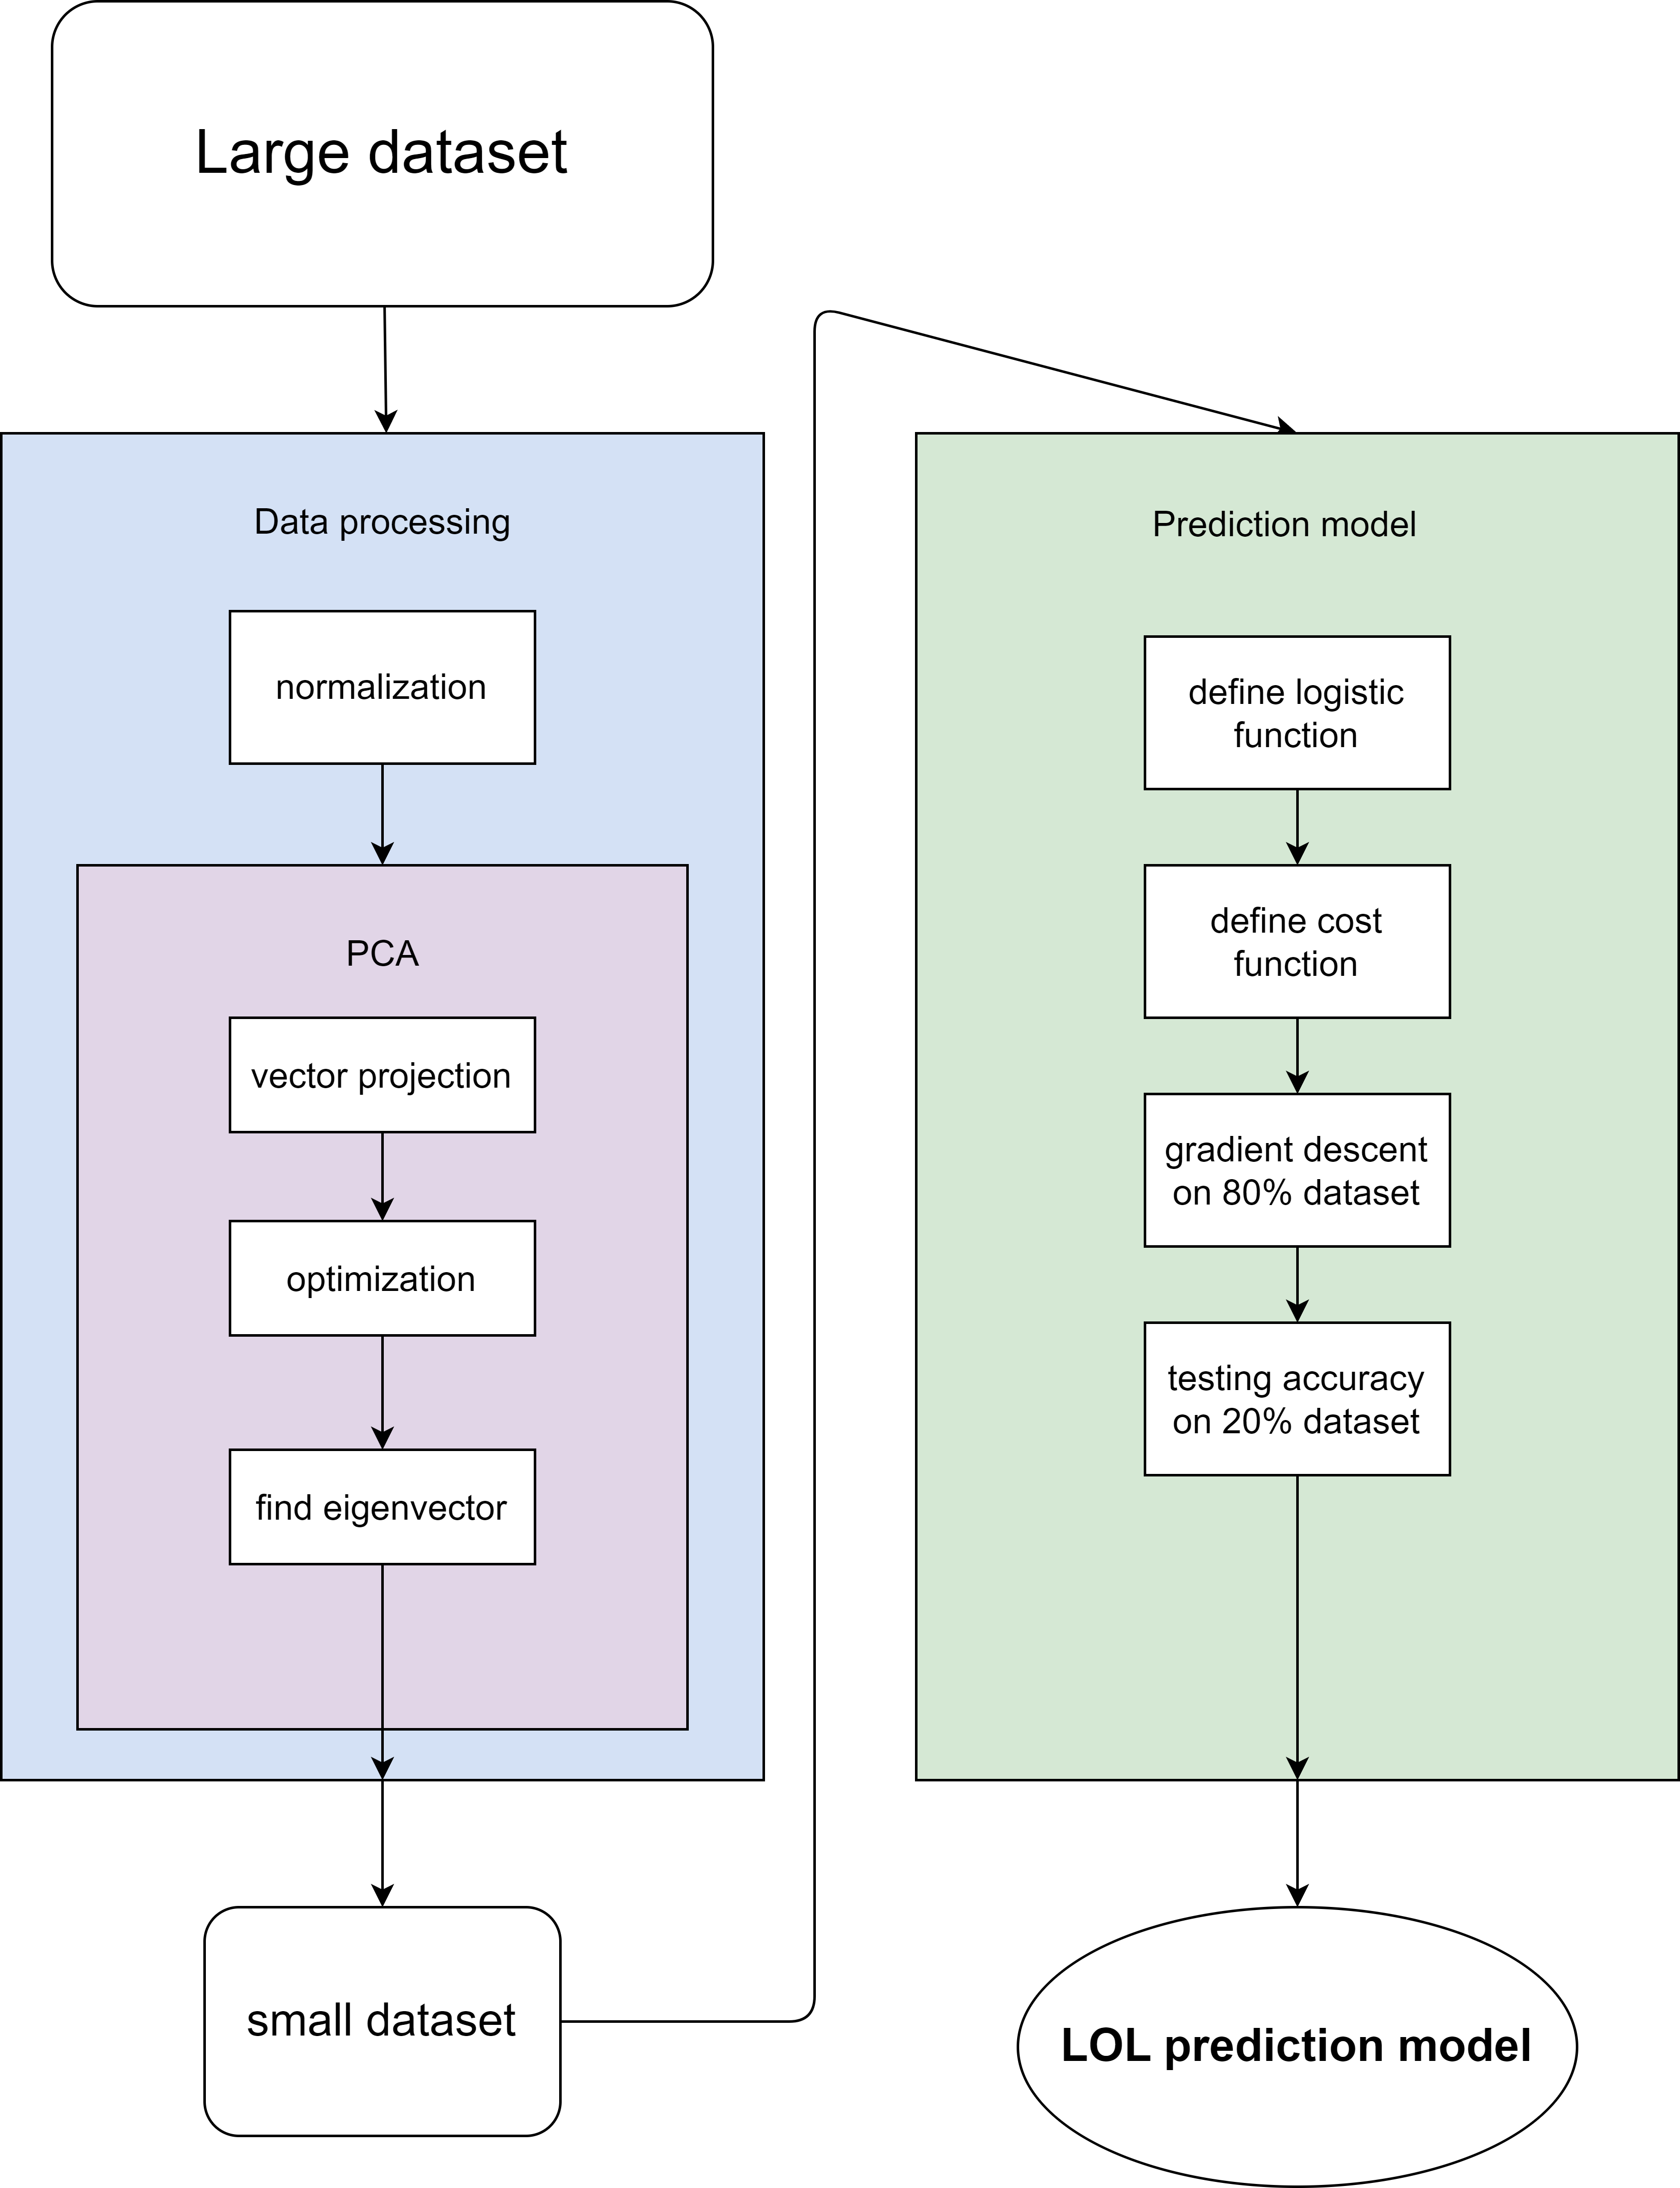
\includegraphics[width=0.6\linewidth]{images/overview-flowchart.png}
    \caption{Overview flowchart}
    \label{fig:overview-flowchart}
\end{figure}




\section{Data}
Thank to the Riot API \parencite{riotgames}, I can access to many game data easily. The data I collected is from LOL ranked games at diamond stage (a stage where most advanced players are at). It contains 9879 games in total and each game with 38 features and one label. Since the whole dataset cannot fit for display, in Table \ref{tab:match-data-snippet}, a $10\times 5$ data snippet is selected from the dataset. The first column, titled "blue wins", contains binary values (only 0 and 1) that indicates whether blue team in this match has eventually won or not. This is called the label for the model that later will be used. Other columns, such as "blue wards placed", "blue first blood" describes the status of teams at the time of 10 minutes. These will be the features, or inputs, of the model.  

\newcolumntype{C}{>{\centering\arraybackslash}p{1.2cm}}
\begin{table}[h]
    \centering
    \caption{A snippet of the match data collected}
    \label{tab:match-data-snippet}
    \begin{tabular}{C|C C C C}
    \toprule
     blue wins &  blue wards placed &  blue wards destroyed &  blue first blood &  blue kills\\
    \midrule
            0 &               28 &                   2 &               1 &          9 \\
            0 &               12 &                   1 &               0 &          5 \\
            0 &               15 &                   0 &               0 &          7 \\
            0 &               43 &                   1 &               0 &          4 \\
            0 &               75 &                   4 &               0 &          6 \\
            1 &               18 &                   0 &               0 &          5 \\
            1 &               18 &                   3 &               1 &          7 \\
            0 &               16 &                   2 &               0 &          5 \\
            0 &               16 &                   3 &               0 &          7 \\
            1 &               13 &                   1 &               1 &          4 \\
    \\ \vdots & \vdots & \vdots & \vdots & \vdots \\
    \bottomrule
    \end{tabular}
\end{table}

\section{Visualizing data}
For better understanding of the data, it can be visualized before diving into modeling.

Currently, the dataset contains 38 features which is large to handle. I need to determine whether they are all useful to the prediction task. Plotting the relationship between features can reveal their usefulness. 

First, let $n$ be the size of a feature. The correlation between two features of length $n$ can be calculated through the Pearson correlation coefficient \parencite{pearson-correlation}. 
\begin{equation}
   r = \frac{\sum (X_i - \bar{X})(Y_i - \bar{Y})}{\sqrt{\sum (X_i - \bar{X})^2 \sum (Y_i - \bar{Y})^2}} 
\end{equation}


The Pearson correlation coefficient is developed by Karl Pearson in 1895. It measures the linear correlation between two sets of data, and gives a normalized data, ranging from $-1$ (perfectly negative correlation) to $1$ (perfectly positive correlation). By calculating for each pair of features, we can plot a correlation heat map indicating the correlation between each pair of data. In the formula, $X_i$ one data point in column $X$, $\bar{X}$ is the mean and the same with column $Y$

\begin{figure}[h]
    \centering
    
\includegraphics[width=0.9\textwidth]{images/heatmap.png}
    \caption{Feature correlation heat map}
    \label{fig:heat-map}
\end{figure}

Since a $38\times 38$ grid is too large for display, I selected 9 features for plotting. In Figure \ref{fig:heat-map}, there is a strong negative correlation between "redFirstBlood" and "blueFirstBlood". This is because in each match there can be only one first blood, either from blue team or red, indicating one of the first blood column is redundant. The "blueGoldPerMin" has a strong positive correlation with "blueKills". This is also reasonable because killing an enemy once will result in gold award. These results shows the dataset is unclean which needs further processing. 

Reducing the dimension (the number of features) of the dataset is important for the modeling process because it makes the model more explainable. 

\section{Data reprocessing}

\subsection{Normalization}
Before reducing the dimension of data, it's necessary to normalize it first. It could be observed from Table \ref{tab:match-data-snippet} that each column are having different ranges. For example the "blue wards placed" has data ranging from 12 to 75 while "blue wards destroyed" only has data ranging from 0 to 4 in the snippet (the range isn't correct for the whole dataset but it's enough for showing the difference between columns). This potentially implies one column with larger values is more important than other columns, which might weaken the accuracy and robustness of the model. Thus we need to normalize the data. 

The standard score of a column can be calculated by: 
\begin{equation}
    x_i=\frac{X_i-\bar{X}}{\sigma}
\end{equation}

where $x_i$ is the new data scaled, $\bar{X}$ is the mean of the column, and $\sigma$ is the standard deviation of the column. This transforms the data to have a mean of 0 and a standard deviation of 1.

\subsection{Principal Component Analysis}
\label{sec:pca}
The most straightforward approach to reduce dimension of data is to remove one of the columns in the strongly correlated pairs. However, this cannot indicate the amount of information lost from our reduction. A more common approach is to use Principal Component Analysis (PCA). 

PCA was developed in 1901, also by Karl Pearson \parencite{pearson-pca}. It's a method to reduce the number of variables in a dataset while keeping the most information.

\subsubsection{Vector projection}

From fig \ref{fig:heat-map} we can see the "blueGoldPerMin" and "blueKills" has strong positive correlation. Here, I'll take these 2 features from the dataset and select only 5 data points from it for illustrating the steps for PCA. For example the column "blue kills" and "blue gold per min":

\begin{figure}[h]
    \centering
    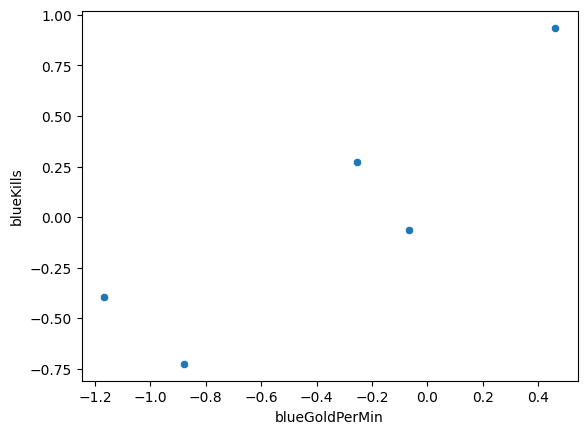
\includegraphics[width=0.8\textwidth]{images/feature-scatter.png}
    \caption{Scatter plot of 2 features}
    \label{fig:feature-scatter}
\end{figure}

We need to find a direction where all of the points will be projected on so that all the 2D points become on one single line, making it 1D. First, for the ease of computation, we express each data point using vectors: 
\begin{equation}
    x_i=
    \begin{bmatrix}
    0.46\\
    0.94
    \end{bmatrix}
\end{equation}

where $x_i$ represent one data point, $1791$ the "blueGoldPerMin" and $9$ "blueKills".

\begin{figure}[h]
    \centering
    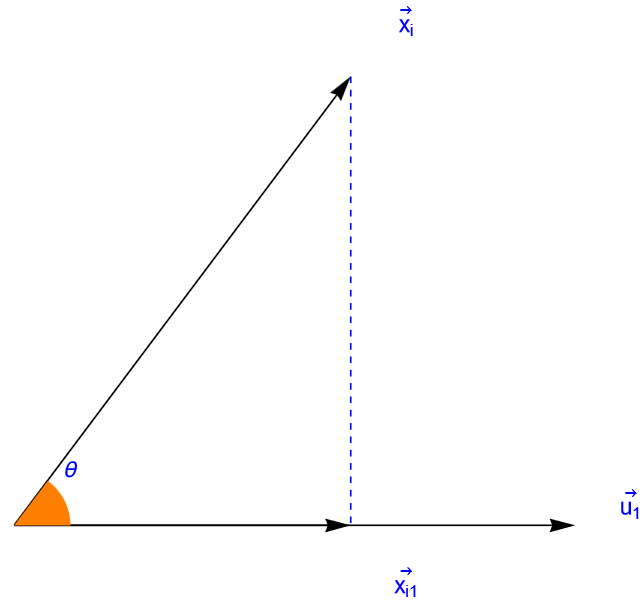
\includegraphics[width=0.6\textwidth]{images/vector-projection.png}
    \caption{Vector projection}
    \label{fig:vector-proejction}
\end{figure}

Next, the projection of the vector $x_i$ onto another direction, represented by a unit vector $u$ with a length of $1$ is illustrated in fig \ref{fig:vector-proejction}. It's mathematically defined:

\begin{equation}
    \label{eq:projection1}
    \frac{|x_i|\cdot \cos \theta}{|u|}
\end{equation}


Because $u$ is a unit vector of length $1$, this means $|u|=1$, so we can simplify the equation \ref{eq:projection1} into:

\begin{equation}
    \label{eq:projection2}
    |x_i|\cdot \cos \theta=|x_i|\cdot 1\cdot \cos \theta=|x_i||u|\cdot \cos \theta
\end{equation}

The benefit of defining $u$ a unit vector is that by equation \ref{eq:projection2}, the projection is equal to the dot product of $x_i$ and $u$. 

\begin{equation}
    \label{eq:projection3}
    |x_i||u|\cdot \cos \theta = x_i\cdot u=x_i^\top  u
\end{equation}




For every data point, we can apply this projection to make all the points lying on the unit vector's vector space, and thus making them 1D. 

\begin{figure}[h]
    \centering
    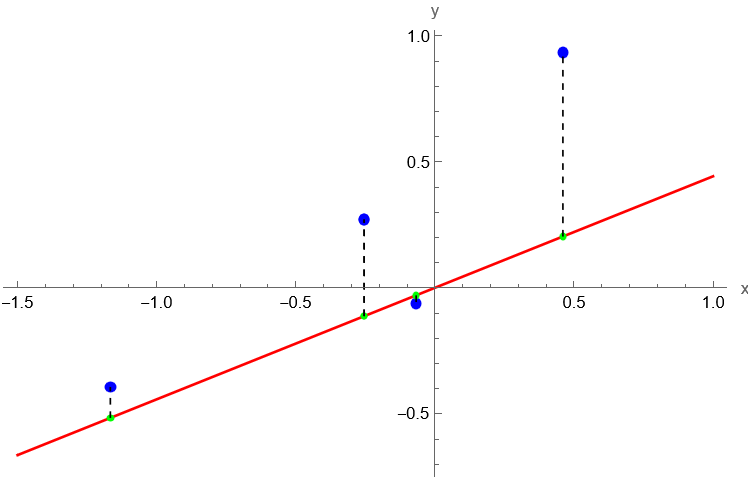
\includegraphics[width=0.8\textwidth]{images/multi-point-projection.png}
    \caption{Projecting all the points}
    \label{fig:multi-point-projection}
\end{figure}

Fig \ref{fig:multi-point-projection} shows the original points (blue) have projected points (green) on the direction of the unit vector's vector space (red). With the process above, we can obtain a new dataset $X_2$

\subsubsection{Vector matrix multiplication}
\label{sec:vector-matrix-multiplication}

In linear algebra, matrix $A$ times vector $v$ can be interpreted as the vector $v$ undergoing a transformation defined by the matrix $A$. 

For example, here we have two base vectors defined:

\begin{gather}
    \label{eq:base-definition}
    i=\begin{bmatrix}
        1 \\ 0
    \end{bmatrix},\ j=\begin{bmatrix}
        0\\1
    \end{bmatrix}
\end{gather}

\begin{figure}[h]
    \centering
    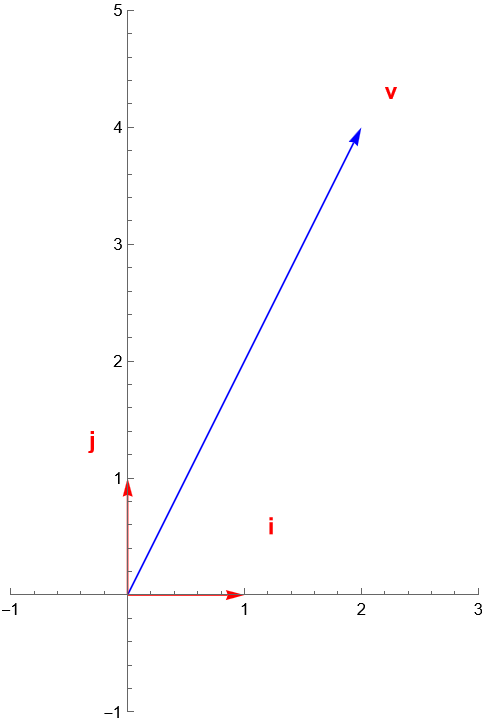
\includegraphics[height=0.8\textwidth]{images/vector1.png}
    \caption{Vector v}
    \label{fig:vector1}
\end{figure}

These two vectors spans the 2D Cartesian plane because for any vector $v$ on it, it can be represented by a linear combination of the two base vectors:

\begin{gather}
    \label{eq:linear-transformation1}
    v=\begin{bmatrix}
        2\\4
    \end{bmatrix}=a\begin{bmatrix}
        1\\0
    \end{bmatrix}+b\begin{bmatrix}
        0\\1
    \end{bmatrix}
    =\begin{bmatrix}
        2\\0
    \end{bmatrix}+
    \begin{bmatrix}
        0\\4
    \end{bmatrix}
\end{gather}

For the matrix $A$:
\begin{gather}
    A=\begin{bmatrix}
        2 & 4\\
        1 & 3
    \end{bmatrix}
\end{gather}

It means that the base vectors have transformed from equation \ref{eq:base-definition} to: 

\begin{gather}
    i=\begin{bmatrix}
        2\\1
    \end{bmatrix},\ j=\begin{bmatrix}
        4\\3
    \end{bmatrix}
\end{gather}    

Similar to the combination in equation \ref{eq:linear-transformation1}, the new vector after the base has changed is now becoming:

\begin{gather}
    \hat{v}=2\begin{bmatrix}
        2\\1
    \end{bmatrix}+4\begin{bmatrix}
        4\\3
    \end{bmatrix}=\begin{bmatrix}
        2\cdot2+4\cdot 4 \\ 1\cdot2+3\cdot4
    \end{bmatrix}=\begin{bmatrix}
        8\\13
    \end{bmatrix}=Av
\end{gather}

\begin{figure}[h]
    \centering
    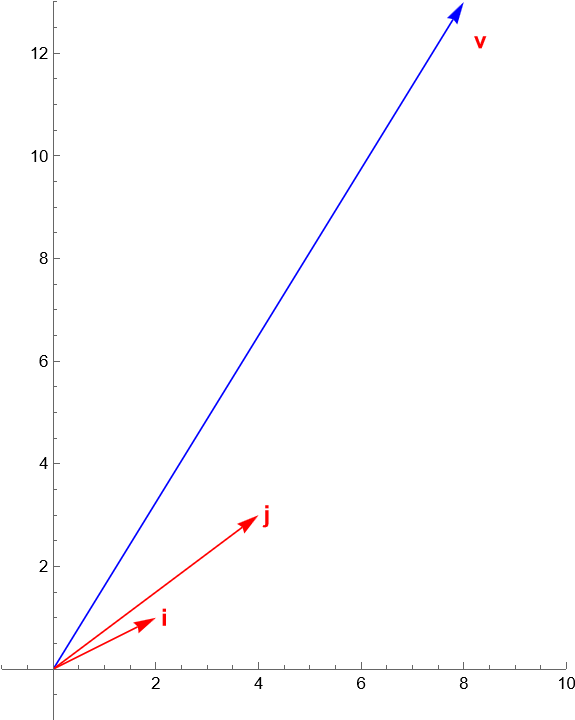
\includegraphics[width=0.6\textwidth]{images/vector2.png}
    \caption{Vector $\hat{v}$}
    \label{fig:vector1}
\end{figure}

\subsubsection{Expressing variance}

Since the aim of PCA is to reduce the dimension of data while maximising the remaining information, this means the green projected points on fig \ref{fig:multi-point-projection} should be as dispersed as possible on the new vector space. We can use variance to measure:

\begin{equation}
    \label{eq:variance1}
    Var(X_2)=\frac{1}{n-1} \sum^n_{i=1} (x_{i2}-\bar{X_2})^2
\end{equation}

where $\bar{X_2}$ is the mean of $X_2$ and $x_i2$ is the element in $X_2$ to differentiate it with $x_i$ in original data. 

Because we have already normalized the data, and transforming it so that it's mean is 0, meaning $\bar{X_2}=0$. Given that the $x_i2$ in $X_2$ is actually calculated above by the projection formula \ref{eq:projection3}. We can transform the equation \ref{eq:variance1} into:
\begin{equation}
    \label{eq:variance2}
    Var(X_2)=\frac{1}{n-1} \sum^n_{i=1} (x_{i2})^2=\frac{1}{n-1}\sum^n_{i=1} (x_i^\top  u)^2
\end{equation}
    
Notice that by expanding $x_i^\top $ it's actually $i$ column vectors $x_i$ that times $u$ as a row vector. This is the same as the definition of matrix vector multiplication.

\begin{gather}
    \sum (x_i^\top  u)^2=
    (\sum
    \begin{bmatrix}
        x_{i1} & x_{i2}
    \end{bmatrix}
    \begin{bmatrix}
        u_1\\
        u_2
    \end{bmatrix})^2\\
    =(Xu)^\top Xu
    =X^\top u^\top Xu
\end{gather}

Substituting this to the formula \ref{eq:variance2}:

\begin{gather}
    Var(X_2)=\frac{1}{n-1}X^\top u^\top Xu
\end{gather}

We can group the matrix terms together:
\begin{gather}
    Var(X_2)=u^\top (\frac{1}{n-1}X^\top X)u
\end{gather}

Because the specific form of the terms in the brackets are unimportant for calculation later, we can simplify it as one term for simpler expression:
\begin{gather}
    C:=\frac{1}{n-1}X^\top X
\end{gather}

Thus, the variation can be simplified:
\begin{gather}
    Var(X_2)=u^\top Cu
\end{gather}

We can express this in a function form:
\begin{gather}
    \label{eq:variance3}
    f(u)=u^\top u
\end{gather}

\subsubsection{Maximum variance}

To maximise the variance, we can find the gradient of function \ref{eq:variance3}. Moreover, since we defined $u$ as a unit vector, and equation \ref{eq:projection2} is based on this definition, the variable $u$ for the function $f(u)$ has a restriction. The following equation describes the task:

\begin{gather}
    \max_{u} u^\top C u \\
    \text{subject to } u^\top u = 1.
\end{gather}

This is a standard optimization problem wit constraints. Without the constraint, we can simply find the $u$ where the gradient of $f(u)$ is equal to $0$. However, given the constraint, we need to use the Lagrange multiplier method.

\subsubsection{Lagrange multiplier method}

Given a function $f(x)$ that needs to be maximised, subject to a constraint $g(x)=c$, where $c$ is a constant. The Lagrangian function is defined:

\begin{gather}
     \mathcal{L}(x, \lambda) = f(x) - \lambda(c-g(x))
\end{gather}
   

where $\lambda$ is a unknown scalar. The term $\lambda(c-g(x))$ can be considered a penalty for the function. In order to minimize the gradient, $c=g(x)$ will mean the constraint is satisfied.

Applying this to our situation, we can set:
\begin{gather}  
    \mathcal{L}(u, \lambda) = f(u) - \lambda(u^\top u-1)\\
    =\mathcal{L}(u, \lambda) = u^\top Cu - \lambda(u^\top u-1)\\
    =\mathcal{L}(u,\lambda)=u^\top Cu+\lambda u^\top u+\lambda
\end{gather}

The function becomes without any constraints, so we can simply maximize it by finding the gradient. For this 2 variable function, the gradient is partial derivative, Because we are aiming to find the $u$, which is the direction where the vectors are mapped are having the greatest variance, we need to find the partial derivative of $\mathcal{L}$ with respect to $u$.

\begin{gather}
    \label{eq:first-partial}
    \frac{\partial f}{\partial u}=2Cu-2\lambda u=0\\
    \label{eq:eigen-form}
    Cu=\lambda u
\end{gather}

However, the derivative only tells the rate of change, when set to $0$, it's a stationary point. We aim to maximize this function, so this stationary point needs to be the maximum point, and thus the function needs to be convex. The detailed proof is in appendix section \ref{sec:convexity}.


\subsubsection{Simplifying eigenvalue equation}
\label{sec:simplifying-eigenvalue-eq}
Looking back at equation \ref{eq:eigen-form}, the left hand side means the base vector has changed according to matrix $C$ on vector $u$. This is equal to the right hand side with a scalar $\lambda$ multiplied by $u$. This means the transformation on the base vector has not impact the direction where vector $u$ is pointing, because scalar vector multiplication only change the magnitude of u. Here the vector $u$ is the eigenvector, and the scalar multiplier $\lambda$ is the eigenvalue. We have $C$ already known, now trying to find vector $u$. 

Here we need to construct a identity matrix $I$ where the top-left to bottom-right diagonal is $1$ and the rest of the elements are $0$.

\begin{gather}
    I=\begin{bmatrix}
        1 & 0\\
        0 & 1
    \end{bmatrix}
\end{gather}

Then it multiplies $\lambda$ will make the diagonal filled with $\lambda$
\begin{gather}
    \lambda I=\begin{bmatrix}
        \lambda & 0\\
        0 & \lambda
    \end{bmatrix}
\end{gather}

\begin{gather}
    \lambda Iu=\begin{bmatrix}
        \lambda & 0\\
        0 & \lambda
    \end{bmatrix} u=\begin{bmatrix}
        \lambda u_1\\
        \lambda u_2
    \end{bmatrix}=\lambda u
\end{gather}

Substituting it into equation \ref{eq:eigen-form}, we get:
\begin{gather}
    Cu=\lambda Iu\\
    (C-\lambda I) u=0\\
\end{gather}

Here $C-\lambda I$ gives a matrix with unknown variable $\lambda$, so it's in the form of matrix vector multiplication. Notice that it's special because the result of multiplication is $0$, which could be written as a vector of zeros:
\begin{gather}
    \label{eq:eigen-equation}
    (C-\lambda I)u=\begin{bmatrix}
        0\\0
    \end{bmatrix}
\end{gather}

This indicates that after the transformation represented by $C-\lambda I$, the eigenvector $u$ shrinks to the origin, have a length of $0$. To solve this equation \ref{eq:eigen-equation}, we need to have a look at what shrinking the eigenvector to the origin mean. 

\subsubsection{Using determinants}
\label{sec:using-determinants}

Determinant for a matrix is, geometrically, a scalar value that gives the area of the parallelogram formed by its column vectors (or the matrix transformed base vectors). We simply denote determinant for a matrix $K$:

\begin{gather}
    K=\begin{bmatrix}
        2 & 1\\
        1 & 2
    \end{bmatrix}\\
    \det (K) = \det\begin{pmatrix}
        2 & 1\\
        1 & 2
    \end{pmatrix}
\end{gather}

Fig \ref{fig:determinant1} illustrate the determinant of $K$. The parallelogram $ABCD$'s area is the determinant of $K$ where $u$ is the first column $[1,2]$ in $K$ and $v$ is the second column $[2,1]$. 

\begin{figure}[h]
    \centering
    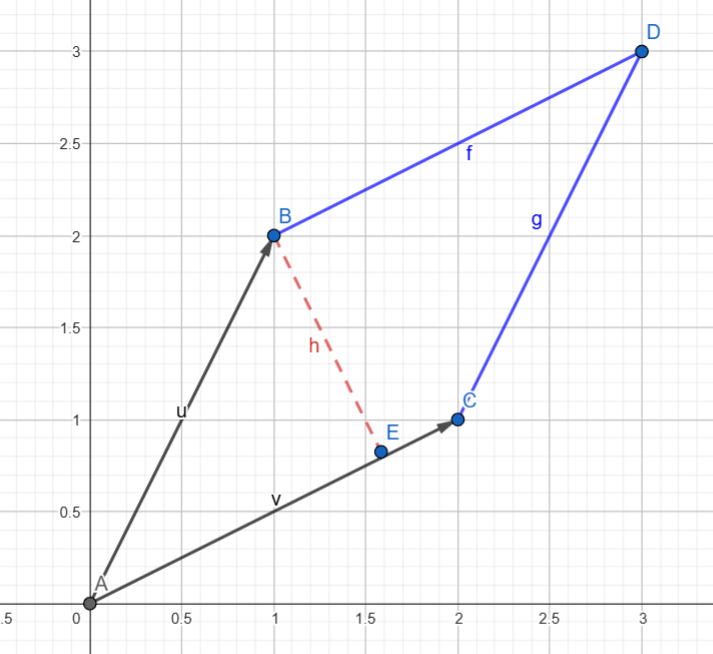
\includegraphics[width=0.7\linewidth]{images/determinant1.png}
    \caption{Illustration of determinant of A}
    \label{fig:determinant1}
\end{figure}

Then the area can be calculated. Draw a perpendicular line $h$ from $B$ to $AC$ which represents the triangle $ABC$'s height. It can be found by using formula for point to a line. By finding the length of $AC$ or the length $|v|$ we can thus calculate the area of triangle $ABC$. Two times the area of $ABC$ is the area of the parallelogram $ABCD$. 

\begin{gather}
    h=\frac{|2\cdot 2-1\cdot 1|}{\sqrt{1^2+2^2}}\\
    =\frac{3}{\sqrt{5}}
\end{gather}

Finding the length of vector $v$:
\begin{gather}
    |v|=\sqrt{1^2+2^2}=\sqrt{5}
\end{gather}

Lastly, find the determinant or the area of the parallelogram:
\begin{gather}
    S_{ABCD}=2\cdot S_{ABC}=2\cdot \frac{1}{2} h |v|\\
    =h|v|=\frac{3}{\sqrt{5}}\cdot \sqrt{5}=3
\end{gather}

We can generalize this process by making $B=(c,d)$, $C=(a,b)$. This represent a matrix $K$:

\begin{gather}
    K=\begin{bmatrix}
        c & a\\
        d & b
    \end{bmatrix}
\end{gather}

Then the determinant of K can be calculated in the same process:

\begin{gather}
    h=\frac{|bc-ad|}{\sqrt{b^2+a^2}}\\
    |v|=\sqrt{b^2+a^2}\\
    S_{ABCD}=|bc-ad|
\end{gather}

However, noting that the area in the determinant is signed, so the absolute value needs to be removed, giving a conclusion when $K$ is 2 by 2:

\begin{gather}
    \det(K)=bc-ad
\end{gather}

This concept also applies to other dimensions of the matrix, but for simplicity in illustrating this process, I chose the dimension of 2. 

\subsubsection{Finding eigenvalue}

Finally, we can find the eigenvalue. Starting with the conclusion in section \ref{sec:simplifying-eigenvalue-eq}, where the transformed eigenvalue shrinks to 0. Expanding the formula \ref{eq:eigen-equation}:

\begin{gather}
    \begin{pmatrix}
        \begin{bmatrix}
        c_1 & c_2\\
        c_3 & c_4
        \end{bmatrix}-\lambda 
        \begin{bmatrix}
        1 & 0\\
        0 & 1
        \end{bmatrix}
    \end{pmatrix}
    \begin{bmatrix}
        u_1\\u_2
    \end{bmatrix}
    =\begin{bmatrix}
        0\\0
    \end{bmatrix}
\end{gather}

Multiplying the scalar $\lambda$ into the identity matrix $I$ gives:
\begin{gather}
    \begin{pmatrix}
        \begin{bmatrix}
        c_1 & c_2\\
        c_3 & c_4
        \end{bmatrix}- 
        \begin{bmatrix}
        \lambda & 0\\
        0 & \lambda
        \end{bmatrix}
    \end{pmatrix}
    \begin{bmatrix}
        u_1\\u_2
    \end{bmatrix}
    =\begin{bmatrix}
        0\\0
    \end{bmatrix}
\end{gather}

Matrix subtraction is simply subtracting each element with corresponding position. Thus the terms in the bracket can be simplified:

\begin{gather}
    \label{eq:eigen-lambda}
    \begin{bmatrix}
        c_1-\lambda & c_2\\
        c_3 & c_4-\lambda
    \end{bmatrix}
    \begin{bmatrix}
        u_1\\u_2
    \end{bmatrix}
    =\begin{bmatrix}
        0\\0
    \end{bmatrix}
\end{gather}

From the conclusion in sub section \ref{sec:using-determinants}, we can conclude that the determinant of the matrix applied to the eigenvector is 0. This is because in section \ref{sec:simplifying-eigenvalue-eq}, we concluded that the eigenvector shrunk to the origin. This means the matrix must have a determinant of 0 because a zero determinant means the transformation collapses the space into a lower dimension, like flattening a 2D object into a point. 

\begin{gather}
    \det 
    \begin{pmatrix}
            \begin{bmatrix}
        c_1-\lambda & c_2\\
        c_3 & c_4-\lambda
    \end{bmatrix}
    \end{pmatrix}=0
\end{gather}

Applying the conclusion from sub subsection \ref{sec:using-determinants}:

\begin{gather}
    (c_1-\lambda)(c_4-\lambda)-c_2c_3=0\\
    \lambda^2-(c_4+c_1)\lambda+c_1c_4-c_2c_3=0
\end{gather}

Given that $C$ is a matrix with known numbers, the only unknown variable is $\lambda$, which is the eigenvalue, and it can be simply found by solving this quadratic equation. 

\begin{gather}
    \lambda = \frac{(c_4+c_1) \pm \sqrt{(c_4-c_1)^2 + 4(c_1c_4-c_2c_3)}}{2}
\end{gather}

Then we can know the matrix in equation \ref{eq:eigen-lambda}. By matrix vector multiplication, we can construct a linear equation:

\begin{gather}
    \begin{cases}
        (c_1-\lambda)u_1+c_2u_2=0\\
        c_3u_1+(c_4-\lambda)u_2=0
    \end{cases}
\end{gather}

By finding the $u_1$ and $u_2$, we can find the eigenvector $u$, which is the direction where all of the data points will be projected to maximise the variance and to minimise the loss of information. This is the whole process of PCA.

\subsection{Applying PCA}

Now, we can apply PCA to the original LOL dataset that has 38 features. 

\begin{figure}[h]
    \centering
    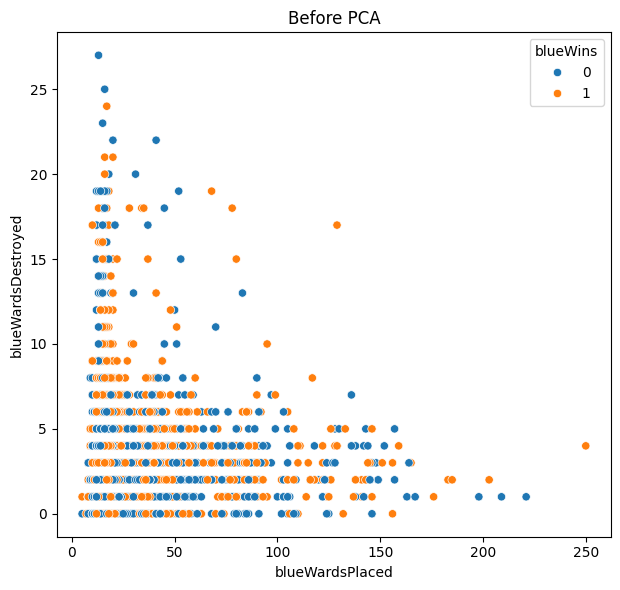
\includegraphics[width=0.7\linewidth]{images/scatter-before-pca.png}
    \caption{Scatter plot of 2 features before PCA}
    \label{fig:scatter-before-pca}
\end{figure}

Fig \ref{fig:scatter-before-pca} shows the scatter plot where orange points suggest blue wins and blue points suggest blue lost. We can compare the scatter plot of 2 features "blueWardsPlaced" and "blueWardsDestroyed" with the scatter plot of 2 features after PCA:

\begin{figure}[h]
    \centering
    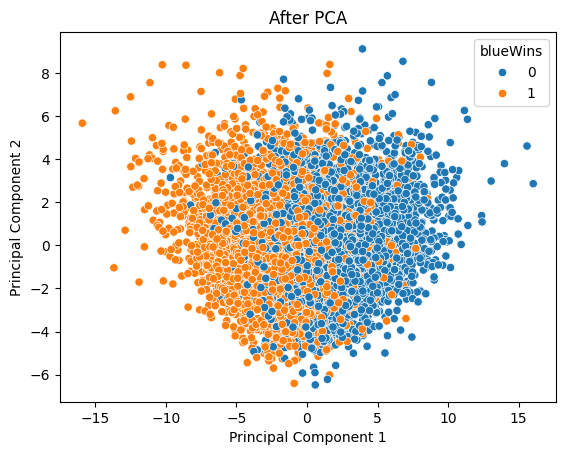
\includegraphics[width=0.7\linewidth]{images/scatter-after-pca.png}
    \caption{Scatter plot of 2 features after PCA}
    \label{fig:scatter-after-pca}
\end{figure}

We can obviously see that the distribution of points is more spacial distinguishable with a general trend of orange points on the left and blue points on the right, much more than fig \ref{fig:scatter-before-pca} before applying PCA. This shows that the useful information is more condensed in only 2 features, derived from the dataset with 38 features. This allows us to apply our prediction model simpler. 

\section{Prediction}
After the data is being processed, we can use models that has the processed features as input and output the prediction. For a binary classification task, logistic regression is well suited.

\subsection{Logistic function}

Logistic regression \parencite{logistic-regression} aims to output a prediction given a set of data. It uses the logistic function in the form:

\begin{gather}
    z=Wx+b\\
    p(z)=\frac{1}{e^{-z}}\\
    p(x)=\frac{1}{e^{-(Wx+b)}}
\end{gather}
with W being the matrix of coefficients, x the vector of input and b a vector of bias.

it looks like this:

\begin{figure}[h]
    \centering
    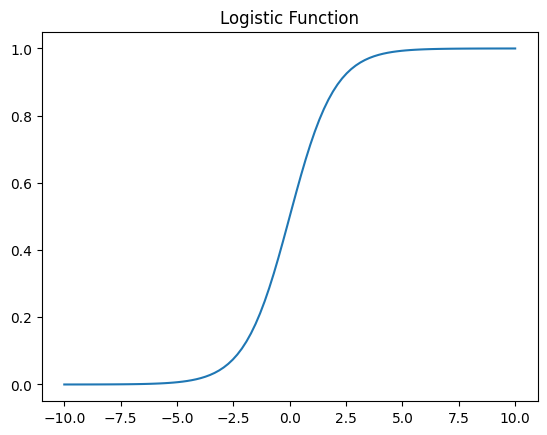
\includegraphics[width=0.6\linewidth]{images/logistic-function.png}
    \caption{Logistic function}
    \label{fig:enter-label}
\end{figure}

There are some properties of this function which explains why it's well fitted for our classification task:

\begin{gather}
    \lim_{z \to \infty} \frac{1}{1 + e^{-z}} = 1\\
    \lim_{z \to -\infty} \frac{1}{1 + e^{-z}} = 0
\end{gather}

This gives the range where $0<f(x)<1$, meaning a probability between blue wins (1) and red wins (0).

So we aim to fit this curve for our dataset and reduce its loss.

\subsection{Evaluating the performance of the model}
In order to train our model with the dataset, we need to first evaluate its current performance. We can define a loss function:

\begin{gather}
    L(f(x),y)=\begin{cases}
        -log(f(x)) & y=1\\
        -log(1-f(x)) & y=0
    \end{cases}
    \label{eq:loss-function1}
\end{gather}

where $y$ is the label. In this case $y$ is the column "blueWins", which is the target output. 

When $y=1$, the loss function is $-log(f(x))$. The output of $f(x)$ should be the closer to $1$ the possible. Thus the greater $f(x)$ is, the loss function $-log(f(x))$ is smaller, and vice versa as shown in fig \ref{fig:loss-function1}.

\begin{figure}[h]
    \centering
    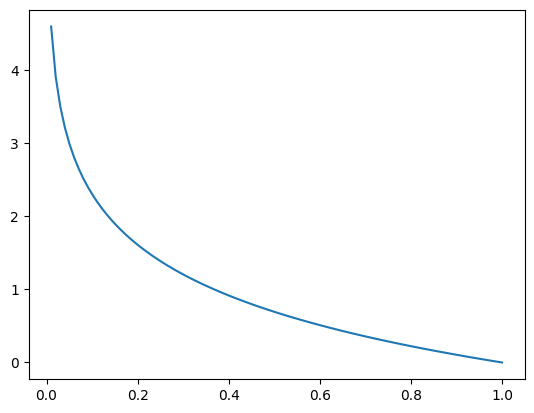
\includegraphics[width=0.5\linewidth]{images/loss-function1.png}
    \caption{Loss function when $y=1$}
    \label{fig:loss-function1}
\end{figure}

When $y=0$, the loss function is $-log(1-f(x))$. The output of $f(x)$ should be the close to $0$ the possible. Thus the smaller $f(x)$ is, the loss function $-log(f(x))$ is smaller, and vice versa as shown in fig \ref{fig:loss-function2}.

\begin{figure}[h]
    \centering
    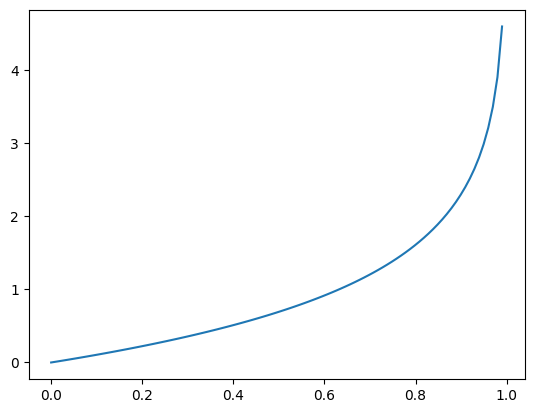
\includegraphics[width=0.6\linewidth]{images/loss-function2.png}
    \caption{Loss function when $y=0$}
    \label{fig:loss-function2}
\end{figure}

We can combine the two separate cost functions into one:

\begin{gather}
    L(f(x),y)=-y\log (f(x))-(1-y)\log (1-f(x))
\end{gather}

This is the same as equation \ref{eq:loss-function1} because when $y=0$, the first term $-y\log (f(x))=0$, only leaving $-(1-y)\log (1-f(x))$, and when $y=1$, the second term $-(1-y)\log (1-f(x))=0$, only leaving $-y\log (f(x))$

Using MSE (mean squared error), we can denote the total cost on the whole dataset:
\begin{gather}
    C(W,b)=-\frac{1}{m}\sum^m_{i=1}[y_i\log(f(x_i))+(1-y_i)\log (1-f(x_i))]
\end{gather}

We can simplify the expression by making the last column vector of $W$ to be $b$

Here we need to optimize the coefficient matrix $W$ to minimize the cost C. We can minimize the partial derivative of $C$ with respect to $W$ to show how the $W$ should change to reduce $C$.

\subsection{Gradient descent}

The gradient gives the way to update the parameter $W$ to reduce the cost function $C$. The gradient is:

\begin{gather}
    \frac{\partial C}{\partial W}=\frac{1}{m}\sum^m_{i=1}(f(x_i)-y_i)x_i
\end{gather}

Every time W reduce the gradient will result in a lower cost:

\begin{gather}
    W_2=W_1-\alpha\frac{\partial C}{\partial W}
\end{gather}

where $\alpha$ is the learning rate, a multiplier that's manually determined for the gradient so that the gradient process can be quicker.

By gradient descent, we can train the logistic model now. However, to accurately evaluate the precision of the model, only $80\%$ of the data will be used, and the other $20\%$ will be used for the validation dataset to ensure that the model is not only working with seen data.

\subsection{Training model}

During gradient descent, the cost of the model reduces in fig \ref{fig:gradient-descent-loss}

\begin{figure}[h]
    \centering
    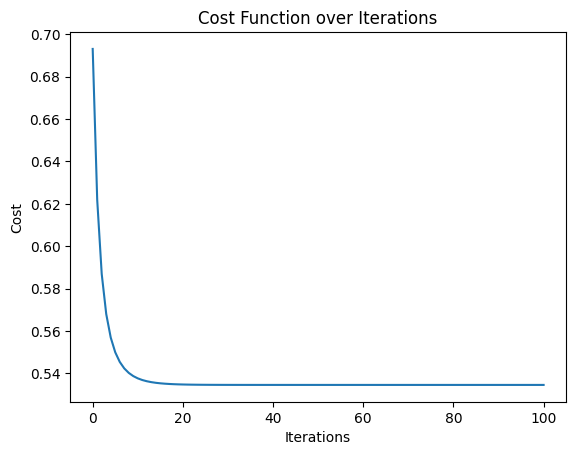
\includegraphics[width=0.6\linewidth]{images/gradient-descent-loss.png}
    \caption{Gradient descent loss}
    \label{fig:gradient-descent-loss}
\end{figure}

As we can see, after 100 iterations, the cost dropped from about $0.7$ to around $0.54$, proving the effectiveness of this process. Moreover, the logistic model now can be visualized on the scatter plot:

\begin{figure}[h]
    \centering
    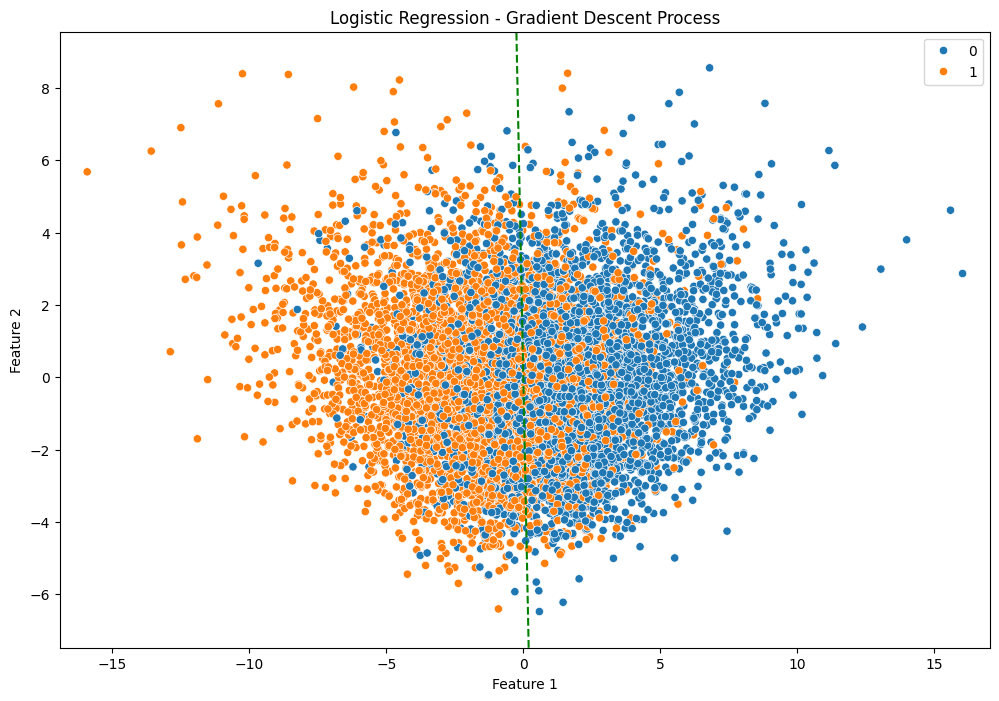
\includegraphics[width=0.8\linewidth]{images/decision-boundary.png}
    \caption{Decision boundary on dataset}
    \label{fig:enter-label}
\end{figure}

where the green line represents the decision boundary that the logistic model draws. It thus categorize the points by their position: on the left of the decision boundary the data will be categorized as blue wins and vice versa.

\subsection{Evaluating model accuracy}

For binary classification task, we can simply use a probability where the prediction value is equal to the real "blueWins" value. By using the model to predict the validation dataset, we can find its accuracy on unseen dataset:

\begin{gather}
    Acc=72.8744939271255\%
\end{gather}

\section{Evaluation}

In this essay, we explored a statistical approach to predicting the outcomes of League of Legends matches using data collected from the Riot API. The methodology employed involved several key steps: data collection, preprocessing, visualization, dimension reduction using Principal Component Analysis (PCA), and building a logistic regression model for prediction.

Overall, the result is, to a large extent, acceptable because competitive games often have many changes and thousands of variables to consider, including the player's mindset that's not quantifiable. Moreover, the dataset only contains the first 10 minute data to predict the winning side, which only gives a trend and ignores everything that happens after 10 minutes. Maybe it's this unpredictability that gives LOL as a competitive game its charm and can remain popular for over 10 years.

However, there are some limitations in the methodology. First, the dataset focused on games at the diamond skill level, which represents a specific subset of League of Legends players. Expanding the analysis to include a wider range of skill levels could provide insights into how the predictive factors vary across different player segments.

Secondly, although PCA condenses the data so that we can visualize and easily operate it, in \ref{sec:pca} there exist information lost when reducing the dimension of the data and though PCA allows for minimum information loss. 

Lastly, the PCA compresses the data. Similar to compressing files, the compressed data cannot be interpreted by human. For example, if applying logistic regression, we can find out what game data, or feature, can impact the result the most and thus explain the result. By compression, we only have access to two feature that have no interpretable relation with LOL data, making the task in this paper specific to purely prediction. 


\printbibliography

\appendix

\section{Additional proofs}

\subsection{Convexity}

\label{sec:convexity}

In single-variable calculus, we use the second derivative test: If $f'(x) = 0$ and $f''(x) < 0$, then $x$ is a local maximum.

Similarly, here we need to find the secondary partial derivative. The secondary partial derivative of formula \ref{eq:first-partial} is:

\begin{gather}
    H=\frac{\partial^2 \mathcal{L}}{\partial u^2} = 2C - 2\lambda I
\end{gather}

Where $H$ is a new matrix called the Hessian matrix. For the function to be convex, it needs to be negative definite, which means for any non-zero vector $v$, we should have:

\begin{gather}
    \label{eq:negative-definite}
    v^\top Hv<0
\end{gather}

Recalling the eigen form in equation \ref{eq:eigen-form}, the matrix $C$ has several eigenvalue, we are typically interested in the largest. The eigenvalue of $C$ are denoted $\lambda_1, \lambda_2, ...,\lambda_n$.

Next, for any non-zero vector $v$, we can express it as a linear combination of eigenvectors of $C$, calling them $k_1,k_2,...,k_n$. We take the largest, making $\lambda=\lambda_1$

\begin{gather}
    v=c_1u_1+c_2u_2+...+c_nu_n
\end{gather}

Now, substituting into the equation \ref{eq:negative-definite}:

\begin{gather}
v^T H v = 2u^\top Cu-2\lambda_1 u^\top u\\
=2(c_1u_1 + ... + c_nu_n)^T C (c_1u_1 + ... + c_nu_n)-2\lambda_1u^\top u
\end{gather}

Because $Cu_i=\lambda_i u_i$,
\begin{gather}
    =2(c_1^2\lambda_1 + c_2^2\lambda_2 + ... + c_n^2\lambda_n)-2\lambda_1u^\top u\\
    =2(c_1^2\lambda_1 + c_2^2\lambda_2 + ... + c_n^2\lambda_n)-2\lambda_1(c_1^2 + c_2^2 + ... + c_n^2)\\
    =2(c_2^2(\lambda_2 - \lambda_1) + c_3^2(\lambda_3 - \lambda_1) + ... + c_n^2(\lambda_n - \lambda_1))
\end{gather}

As we can see, for each term, there is one $\lambda_i -\lambda_1$, because $\lambda_1$ is the largest, so $\lambda_i-\lambda_1$ is negative, and making the whole expression negative, in2dicating that the Hessian matrix $H$ is negative definite. Thus, we had proven the convexity of the function $\mathcal{L}$.

\section{Python Codes}
\label{sec:python-codes}
\subsection{Setup}
\begin{lstlisting}[style=pythonstyle]
# imports
import numpy as np
import matplotlib.pyplot as plt
import seaborn as sns
import pandas as pd

# import csv
raw_data=pd.read_csv('rank-data/high_diamond_ranked_10min.csv').dropna()
raw_data.info()

raw_data.head()
\end{lstlisting}

\subsection{Plotting heatmap}
\begin{lstlisting}[style=pythonstyle]
raw_data.drop('gameId',axis=1,inplace=True)
raw_data.head()
raw_data

# plot heat map
selected_columns = raw_data.columns[1:5].tolist()+raw_data.columns[18:23].tolist()
selected_df = raw_data[selected_columns]
corr_matrix=selected_df.corr()
sns.heatmap(corr_matrix,
            # annot=True,
            cmap='coolwarm')
plt.figure(figsize=(20,10))
plt.show()
\end{lstlisting}

\subsection{Normalization}
\begin{lstlisting}[style=pythonstyle]
from sklearn.preprocessing import StandardScaler
from sklearn.decomposition import PCA

scaler = StandardScaler()
scaled_features=scaler.fit_transform(features)

pca=PCA(n_components=2)
principal_components=pca.fit_transform(scaled_features)
feature_pca=pd.DataFrame(data=principal_components)
feature_pca.head()
#convert scaled features to dataframe
scaled_features=pd.DataFrame(data=scaled_features,columns=features.columns)
\end{lstlisting}

\subsection{Comparison scatter plot}
\begin{lstlisting}[style=pythonstyle]
plt.figure(figsize=(12, 6))

# Before PCA
plt.subplot(1, 2, 1)
sns.scatterplot(x=features.iloc[:, 0], y=features.iloc[:, 1], hue=raw_data['blueWins'])
plt.title('Before PCA')
plt.xlabel('blueWardsPlaced')
plt.ylabel('blueWardsDestroyed')

# plt.subplot(1, 2, 2)
# sns.scatterplot(x=selected_features.iloc[:, 0], y=selected_features.iloc[:, 1], hue=raw_data['blueWins'])
# plt.title('Before PCA')
# plt.xlabel('blueDeaths')
# plt.ylabel('redTotalGold')

plt.tight_layout()
plt.show()

# After PCA
sns.scatterplot(x=feature_pca[0], y=feature_pca[1], hue=raw_data['blueWins'])
plt.title('After PCA')
plt.xlabel('Principal Component 1')
plt.ylabel('Principal Component 2')

\end{lstlisting}

\subsection{Logistic regression}
\begin{lstlisting}[style=pythonstyle]
from sklearn.model_selection import train_test_split

# X_train, X_test, y_train, y_test = train_test_split(feature_pca, label, test_size=0.2, random_state=42)
X_train, X_test, y_train, y_test = train_test_split(feature_pca, label, test_size=0.2, random_state=42)

X_train.shape,X_test.shape,y_train.shape,y_test.shape

from sklearn.metrics import accuracy_score, confusion_matrix, classification_report

from sklearn.linear_model import LogisticRegression
# fit the model
log_reg = LogisticRegression()
log_reg.fit(X_train, y_train)
log_reg_pred = log_reg.predict(X_test)
# accuracy
log_reg_accuracy = accuracy_score(y_test, log_reg_pred)
log_reg_accuracy
\end{lstlisting}

\subsection{Plotting decision boundary on scatterplot}
\begin{lstlisting}[style=pythonstyle]
import numpy as np
import matplotlib.pyplot as plt

X=X_train.values
y=y_train.values

# Sigmoid function
def sigmoid(z):
    return 1 / (1 + np.exp(-z))

# Logistic regression with gradient descent
def logistic_regression(X, y, learning_rate=0.1, num_iterations=1000):
    m, n = X.shape
    theta = np.zeros(n)
    theta_history = []

    for i in range(num_iterations):
        z = np.dot(X, theta)
        h = sigmoid(z)
        gradient = np.dot(X.T, (h - y)) / m
        theta -= learning_rate * gradient
        
        if i % 100 == 0:  # Store theta every 100 iterations
            theta_history.append(theta.copy())
    
    return theta, theta_history

# Run logistic regression
theta, theta_history = logistic_regression(X, y)

# Plotting
plt.figure(figsize=(12, 8))

# Plot the data points
sns.scatterplot(x=X[:, 0], y=X[:, 1], hue=y)
# sns.scatterplot(x=[:, 0], y=[:, 1],hue=y_train)
# plt.scatter(X[y==1][:, 0], X[y==1][:, 1], c='r', label='Class 1')

# Plot decision boundaries at different iterations
x1_min, x1_max = X[:, 0].min() - 1, X[:, 0].max() + 1
x2_min, x2_max = X[:, 1].min() - 1, X[:, 1].max() + 1
xx1, xx2 = np.meshgrid(np.arange(x1_min, x1_max, 0.01),
                       np.arange(x2_min, x2_max, 0.01))

for i, theta in enumerate(theta_history):
    Z = sigmoid(np.c_[xx1.ravel(), xx2.ravel()].dot(theta))
    Z = Z.reshape(xx1.shape)
    
    # plot if on last iterations
    if i == len(theta_history) - 1:
        plt.contour(xx1, xx2, Z, [0.5], colors=['g'], 
                    linestyles=['--'], 
                    label=f'Iteration {i*100}')

plt.xlabel('Feature 1')
plt.ylabel('Feature 2')
plt.title('Logistic Regression - Gradient Descent Process')
plt.legend()
plt.show()
\end{lstlisting}

\end{document}

%% 
%% Copyright (C) 2019 by Daniel A. Weiss <daniel.weiss.led at gmail.com>
%% 
%% This work may be distributed and/or modified under the
%% conditions of the LaTeX Project Public License (LPPL), either
%% version 1.3c of this license or (at your option) any later
%% version.  The latest version of this license is in the file:
%% 
%% http://www.latex-project.org/lppl.txt
%% 
%% Users may freely modify these files without permission, as long as the
%% copyright line and this statement are maintained intact.
%% 
%% This work is not endorsed by, affiliated with, or probably even known
%% by, the American Psychological Association.
%% 
%% This work is "maintained" (as per LPPL maintenance status) by
%% Daniel A. Weiss.
%% 
%% This work consists of the file  apa7.dtx
%% and the derived files           apa7.ins,
%%                                 apa7.cls,
%%                                 apa7.pdf,
%%                                 README,
%%                                 APA7american.txt,
%%                                 APA7british.txt,
%%                                 APA7dutch.txt,
%%                                 APA7english.txt,
%%                                 APA7german.txt,
%%                                 APA7ngerman.txt,
%%                                 APA7greek.txt,
%%                                 APA7czech.txt,
%%                                 APA7turkish.txt,
%%                                 APA7endfloat.cfg,
%%                                 Figure1.pdf,
%%                                 shortsample.tex,
%%                                 longsample.tex, and
%%                                 bibliography.bib.
%% 
%%
%%
%% This is file `./samples/shortsample.tex',
%% generated with the docstrip utility.
%%
%% The original source files were:
%%
%% apa7.dtx  (with options: `shortsample')
%% ----------------------------------------------------------------------
%% 
%% apa7 - A LaTeX class for formatting documents in compliance with the
%% American Psychological Association's Publication Manual, 7th edition
%% 
%% Copyright (C) 2019 by Daniel A. Weiss <daniel.weiss.led at gmail.com>
%% 
%% This work may be distributed and/or modified under the
%% conditions of the LaTeX Project Public License (LPPL), either
%% version 1.3c of this license or (at your option) any later
%% version.  The latest version of this license is in the file:
%% 
%% http://www.latex-project.org/lppl.txt
%% 
%% Users may freely modify these files without permission, as long as the
%% copyright line and this statement are maintained intact.
%% 
%% This work is not endorsed by, affiliated with, or probably even known
%% by, the American Psychological Association.
%% 
%% ----------------------------------------------------------------------